\section{Execution of instruccions}

\subsection{The concept of `executing only if resources available'}
When decoded, a particular instruccion will only be executed if the resources used by the instruction are available.

Availability of resources means that source and destination operands and the corresponding execution unit are free
to perform the instruction execution. Otherwise, the instruction will be stalled till all resources are available.
This mechanism ensures that all instruction are always properly executed.

\subsection{ALU}
\textcolor{red}{Esto debería sacarse de acá}
The integer arithmetic logic unit (ALU) operates on 32 and 64 bits integer data sources and result. It also needs to
report carry, overflow, zero and negative flags. The ALU is in charge of all arithmetic and logic operations on GPR's.

\begin{table}
\begin{center}
\begin{tabu}{|X[l]|X[3,l]|X[c]|X[c]|}
\hline
\rowfont[c]\bfseries
Port name & Description & Size (Bits) & Type\\
\hline
\hline
clk                & Posedge active clock                         & 1  & Input   \\
\hline
start              & High active strobe start execution           & 1  & Input   \\
                   & Note: This signal must be implemented only for a non-pipelined ALU. & 1  & Input   \\
\hline
rst                & High active asynchronous reset               & 1  & Input   \\
\hline
srst               & High active synchronous reset                & 1  & Input   \\
\hline
ena		   & High active synchronous enable		  & 1  & Input \\
\hline
format             & Word or long word operands                   & 2  & Input   \\
                   & '0': Word                                    &    &         \\
                   & '1': Long                                    &    &         \\
\hline
operation          & Selects the operation to be executed         & XX & Input   \\
\hline
operand\_x         & First operand                                & 64 & Input   \\
\hline
operand\_y         & Second operand                               & 64 & Input   \\
\hline
flags              & Ouptut flags                                 & 3  & Output  \\
                   & Bit 0: zero                                  &    &         \\
                   & Bit 1: overflow                              &    &         \\
                   & Bit 2: carry                                 &    &         \\
                   & Note: Negative flag is implicit (MSB of the result) &    &         \\
\hline
result             & Operation result                             & 64 & Output  \\
\hline
done               & Up when finished and until start is asserted & 1  & Output  \\     
                   & Note: This signal must be implemented only for a non-pipelined ALU. & 1  & Input   \\
\hline
\end{tabu}
\end{center}
\caption{ALU Port interface}
\label{tbl:alu_interface}
\end{table}

\subsection{Floating point unit}
\textcolor{red}{Esto debería sacarse de acá}
The floating point unit (FPU) is optional to the design. The FPU is in charge of all arithmetic and logic operations on FPR's
operating on 32 and 64 bits formats.

When FPU is not provided, floating point operations must always generate
an exception and the corresponding exception mask should not be set. In this case, software support must be provided to handle the
exception and returning a consistent result, so the execution of the program can be resumed. Read section \ref{sec:exceptions} for more
information.

If the optional FPU is present, it must be IEEE 754 compliant and provide the following interface.

\begin{table}
\begin{center}
\begin{tabu}{|X[l]|X[3,l]|X[c]|X[c]|}
\hline
\rowfont[c]\bfseries
Port name & Description & Size (Bits) & Type\\
\hline
\hline
clk                & Posedge active clock                         & 1  & Input   \\
\hline
start              & High active strobe start execution           & 1  & Input   \\
                   & Note: This signal must be implemented only for a non-pipelined FPU. & 1  & Input   \\
\hline
rst                & High active asynchronous reset               & 1  & Input   \\
\hline
srst               & High active synchronous reset                & 1  & Input   \\
\hline
ena		   & High active synchronous enable		  & 1  & Input \\
\hline
fp\_format         & Single or double precission operands         & 2  & Input   \\
                   & '0': Single                                  &    &         \\
                   & '1': Double                                  &    &         \\
\hline
rnd\_mode          & Establishes rounding mode for the result     & 2  & Input   \\
                   & '00': RN - Round to nearest                  &    &         \\
                   & '01': RZ - Round towards zero                &    &         \\
                   & '10': RP - Round towards plus infinity       &    &         \\
                   & '11': RM - Round towards minus infinity      &    &         \\
\hline
operation          & Selects the operation to be executed         & XX & Input   \\
\hline
operand\_x         & First operand                                & 64 & Input   \\
\hline
operand\_y         & Second operand                               & 64 & Input   \\
\hline
cause              & Exception cause                              & 4  & Output  \\
                   & Bit 0: Underflow                             &    &         \\
                   & Bit 1: Overflow                              &    &         \\
                   & Bit 2: Division by zero                      &    &         \\
                   & Bit 3: Invalid operation                     &    &         \\
\hline
flags              & Ouptut flags                                 & 3  & Output  \\
                   & Bit 0: Zero                                  &    &         \\
                   & Bit 1: Infinity                              &    &         \\
                   & Bit 2: A number                              &    &         \\
                   & Note: Negative flag is implicit (MSB of the result) &    &         \\
\hline
result             & Operation result                             & 64 & Output  \\
\hline
done               & Up when finished and until start is asserted & 1  & Output  \\
                   & Note: This signal must be implemented only for a non-pipelined FPU. & 1  & Input   \\
\hline
\end{tabu}
\end{center}
\caption{ALU Port interface}
\label{tbl:fpu_interface}
\end{table}

\subsection{FPU timig diagrams}
\begin{figure}
\begin{center}
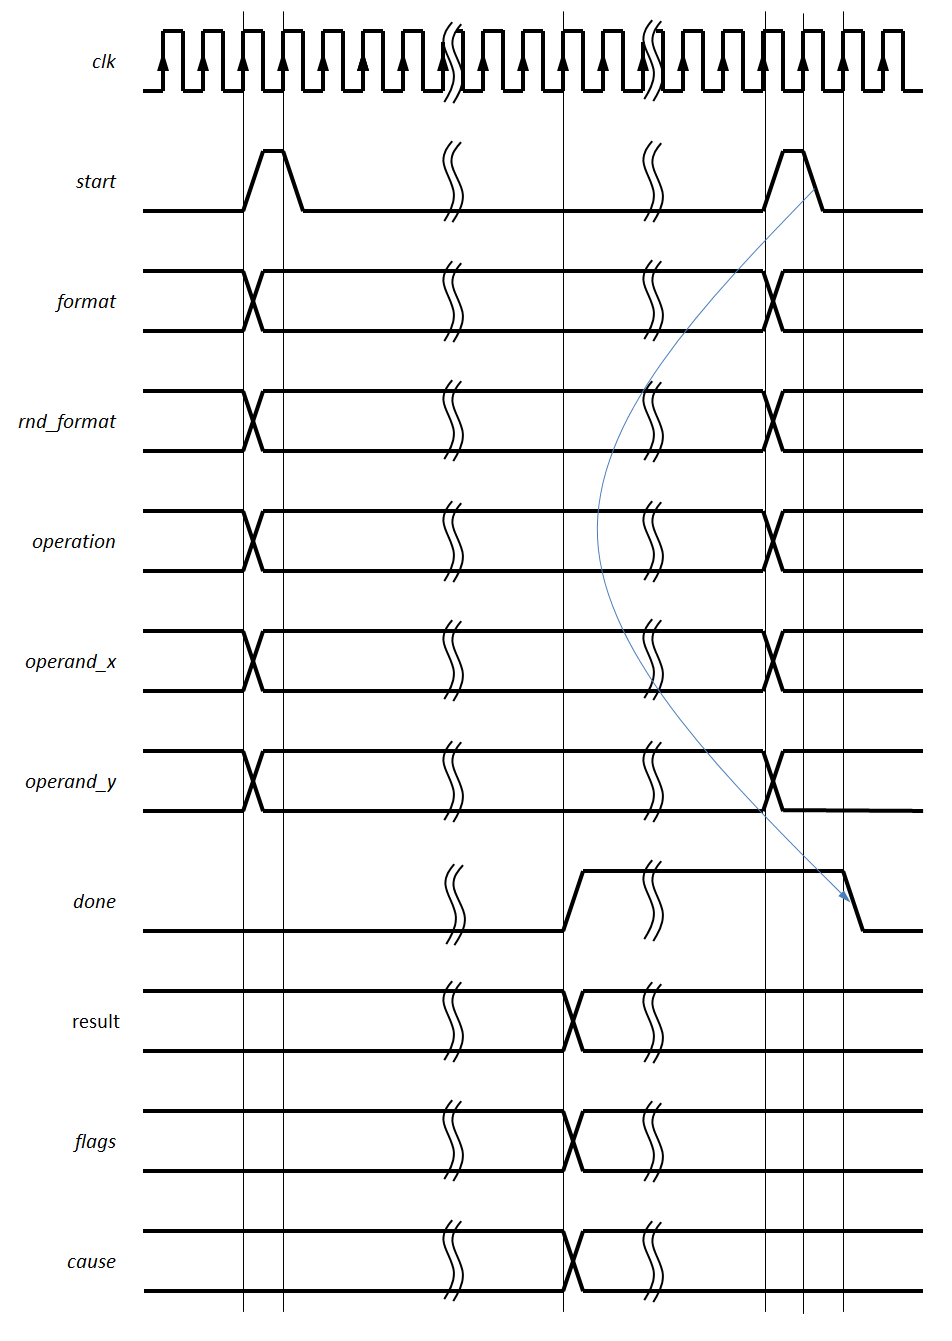
\includegraphics[scale=0.35]{./figures/fpu_timing.png}
\end{center}
\caption{FPU timing diagram.}
\label{fig:fpu_timing}
\end{figure}
